\documentclass{ctexart}
\usepackage{float}
\usepackage{pifont}
\usepackage{multirow}
\usepackage{array}
\usepackage{amsmath}
\usepackage{amssymb}
\usepackage{graphicx}
\usepackage{gbt7714}
\usepackage{wrapfig}
\ctexset{
    % 修改 section。
    section={   
        name={,、},
        number={\chinese{section}}
    }
}

\title{在气垫导轨上研究阻尼振动}
\author{陆知辰-10225301478}
\date{\today}
\graphicspath{{figure/}}

\begin{document}

\begin{titlepage}
  \centering
  % 插入图片
  
\includegraphics[width=0.5\textwidth]{ecnu.png}
  
  % 空行用于调整标题位置
  \vspace*{\baselineskip}
  
  % 标题
  \Huge\textbf{物\quad 理\quad 实\quad 验 \quad (二)}
  % 空行用于调整标题和其他信息之间的间距
  \vspace*{0.3\baselineskip}
  
  % 具体实验名称
  \huge 在气垫导轨上研究阻尼振动
  
  % 空行用于调整时间和其他信息之间的间距
  \vspace*{2\baselineskip}
  
  % 时间
  \large 时间:\today
  
  % 空行用于调整时间和其他信息之间的间距
  \vspace*{\baselineskip}
  
  % 创作人
  \large 创作人:陆知辰
  
  % 空行用于调整创作人和学号之间的间距
  \vspace*{\baselineskip}
  
  % 学号
  \large 学号:10225301478
  
\end{titlepage}
\newpage
\tableofcontents
\newpage
\section{摘要}
简谐振动是周期运动中最简单的运动方式。研究简谐振动是了解周期运动最简单最理想的模型。
而当简谐振动中加入了和速度相关的粘性阻力的时候,振动将变为阻尼振动。

本实验通过在气垫导轨上更换弹簧与配重获得不同实验条件,通过视频记录与数据记录获得不同周期中最大振幅数据,并进行数据处理
得到在最大振幅处不同弹簧弹性系数与滑块质量下的若干周期的图像。
并计算不同条件下的粘性阻尼系数与品质因数。\\
\newline
\textbf{关键词:} \quad 气垫导轨、阻尼振动、品质因数、弹性系数、粘性阻尼系数

\section{原理}
  \subsection{背景知识}
  \begin{figure}[H]
    \centering
    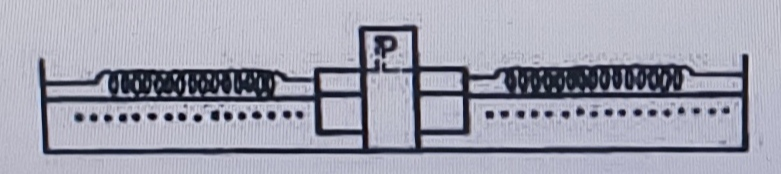
\includegraphics[width=0.8\textwidth,height=0.1\textheight]{yuanlitu.jpg}
    \caption{阻尼振动原理图}
    \label{yuanlitu}
  \end{figure}

  本实验的阻尼谐振子由气垫导轨上的滑块和一对弹簧组成,如图\ref{yuanlitu}
  此时滑块除受弹簧恢复力作用外,还受到滑块与导轨之间的粘性阻力的作用。在滑块速度较小时,粘性阻力$F_{\mbox{阻}}$和滑块的速度成正比,即

  \begin{equation}
    F_{\mbox{阻}} = bv =b \frac{dx}{dt}
  \end{equation}


  式中b为粘性阻尼常量。气垫导轨上由滑块和一对弹簧组成的振动系统,在弹性力kx和阻尼力$F_{\mbox{阻}}$作用下,滑块的运动方程为

  \begin{equation}
    m \frac{d^{2}x}{dt^{2}} = -kx - b\frac{dx}{dt}
  \end{equation}

  式中m为滑块质量,令

  $$2\delta = \frac{b}{m}, \omega^{2}_{0} = \frac{k}{m}$$

  其中$\delta$为阻尼因素,$\omega_{0}$为振动系统固有频率。由此,可以得到

  \begin{equation}
    m \frac{d^{2}x}{dt^{2}} + 2\delta \frac{dx}{dt} + \omega^{2}_{0} x = 0
  \end{equation}

  当阻力较小的时候,该方程的解为

  \begin{equation}
    x = A_{0} e^{-\delta t} \cos (\omega_{f} t + \phi)
  \end{equation}

  其中$\omega_{f} = \sqrt[2]{\omega_{0}^{2} - \delta^{2}}$,而阻尼振动的周期为

  $$T = \frac{2\pi}{\omega_{f}} = \frac{2\pi}{\sqrt{\omega_{0}^{2} - \delta^{2}}}$$

  由此可以得到阻尼振动主要特点

  阻尼振动振幅随着时间按指数规律衰减,也就是$A=A_{0} e^{-\delta t}$。而衰减速度除了时间相关,还和阻尼因素相关,也就是和$\delta=\frac{b}{2m}$,所以也和粘性阻尼常数b以及质量m相关。

  \subsection{进一步计算}
    \subsubsection{阻尼常数/粘性阻尼常数计算}
    将某一时刻的振幅和一个周期之后该位置的振幅进行比值计算,将会得到

    \begin{equation}
      \Delta = \frac{A_{0} e^{\delta t}}{A_{0} e^{\delta (t+T)}}
    \end{equation}

    再将该值取对数,将会得到

    \begin{equation}
      \Lambda = \ln \Delta = \ln \frac{A_{0} e^{\delta t}}{A_{0} e^{\delta (t+T)}} = \delta T
    \end{equation}

    若将$\delta = \frac{b}{2m}$代入,则会得到

    \begin{equation}
      b = \frac{2m\Lambda}{T}
    \end{equation}

    由此可以得到$\delta$或者b,需要测量的质量以及周期以及振幅数据。

    \subsubsection{品质因数}
    一个振动系统的品质因素又称Q值,是一个应用极为广泛的概念,它在交流电系统及无线电电子学中是一个很常见的术语。
    品质因数是指振动系统的总能量E与在一个周期中所损耗的能量$\Delta E$之比的$2\pi$倍,用Q表示,也就是

    \begin{equation}
      Q=2\pi \frac{E}{\Delta E}
    \end{equation}

    阻尼振动中,能量的损耗是由于克服阻尼力作功而造成的,其作功的功率等于阻尼力的大小bv乘以运动速率v,即等于$bv^{2}$。
    在振动时,$bv^{2}$是一个变量,可用一个周期中的平均值作为这一周期中的平均效果。
    这样,一个周期中的能量损耗$\Delta E$等于一个周期中克服阻尼力作的功,即

    $$\Delta E = (bv^{2})_{\mbox{平均}}T$$

    而对于振动系统而言,一个周期中的平均动能等于平均势能,且均等于总能量的一半。所以可以得到

    \begin{equation}
      (\frac{1}{2}mv^{2})_{\mbox{平均}} = (\frac{1}{2}kx^{2})_{\mbox{平均}} = \frac{1}{2} E
    \end{equation}

    \begin{equation}
      (v^{2})_{\mbox{平均}} = \frac{E}{m}
    \end{equation}

    \begin{equation}
      \Delta E = b \frac{E}{m} T
    \end{equation}
    
    最终可以得出$Q = \frac{\pi}{\Lambda}$

  \subsection{实验所需测量量}
  实验中所需要测量$\Lambda$,也就是需要得到某一位置的振幅,以及一个周期之后该位置的振幅。所以实验中选取振幅最大值的位置为观察位置
  进行测量观测。

  并通过描点观察振幅变化和周期变化。最终计算品质因数。


\section{装置器材}
气垫导轨,滑块,摄像仪器,弹簧数对,重物质量块,物理天平,米尺

\section{内容及步骤}
  \subsection{系统调节}
  安装完光电门传感器后测试光电门计时功能是否正常使用再进行导轨水平调整。
  导轨的水平调节通过导轨一端安装的调节螺丝,用于调节导轨横向与纵向的水平。
  在调节水平的时候通过结合静态调节和动态调节的方式进行调节。
    \subsubsection{静态调节}
    打开气源开关,将滑块放于导轨任意位置,观察滑块是否会发生滑动。反复多次
    调节底部螺丝,直到滑块保持不动,或稍有移动但无一定方向性为止。应选择多个
    位置进行试验。
    \subsubsection{动态调节}
    原理是如果滑块已经调平,则通过导轨任意位置的速度应该相同,滑块作匀速直线
    运动。所以在滑块通过两个光电门的时候的速度应该是相等的。所以以一定初速度
    释放滑块记录滑块通过两个光电门的速度大小并作出相应的调节,最终使得滑块通过
    两光电门的速度相差不超过5\%。
  \subsection{弹簧弹力系数测量}
  测量弹簧原本长度,在悬挂质量块后再次测量长度,多次悬挂不同质量的重物测量弹簧的型变量,通过计算得到
  弹簧的弹性系数。导轨弹簧弹性系数等于两侧弹簧弹性系数的和,即$k_{\mbox{总}}=k_{1}+k_{2}$。
  \subsection{振幅测量}
  选择不同弹性系数的弹簧组合,在某一位置释放小车,并通过改变小车的负重改变总质量进行多次实验。

  通过视频方式记录小车位置,再对视频进行在处理得到数据集。
\newpage

\section{原始数据}
\begin{figure}[H]
  \centering
  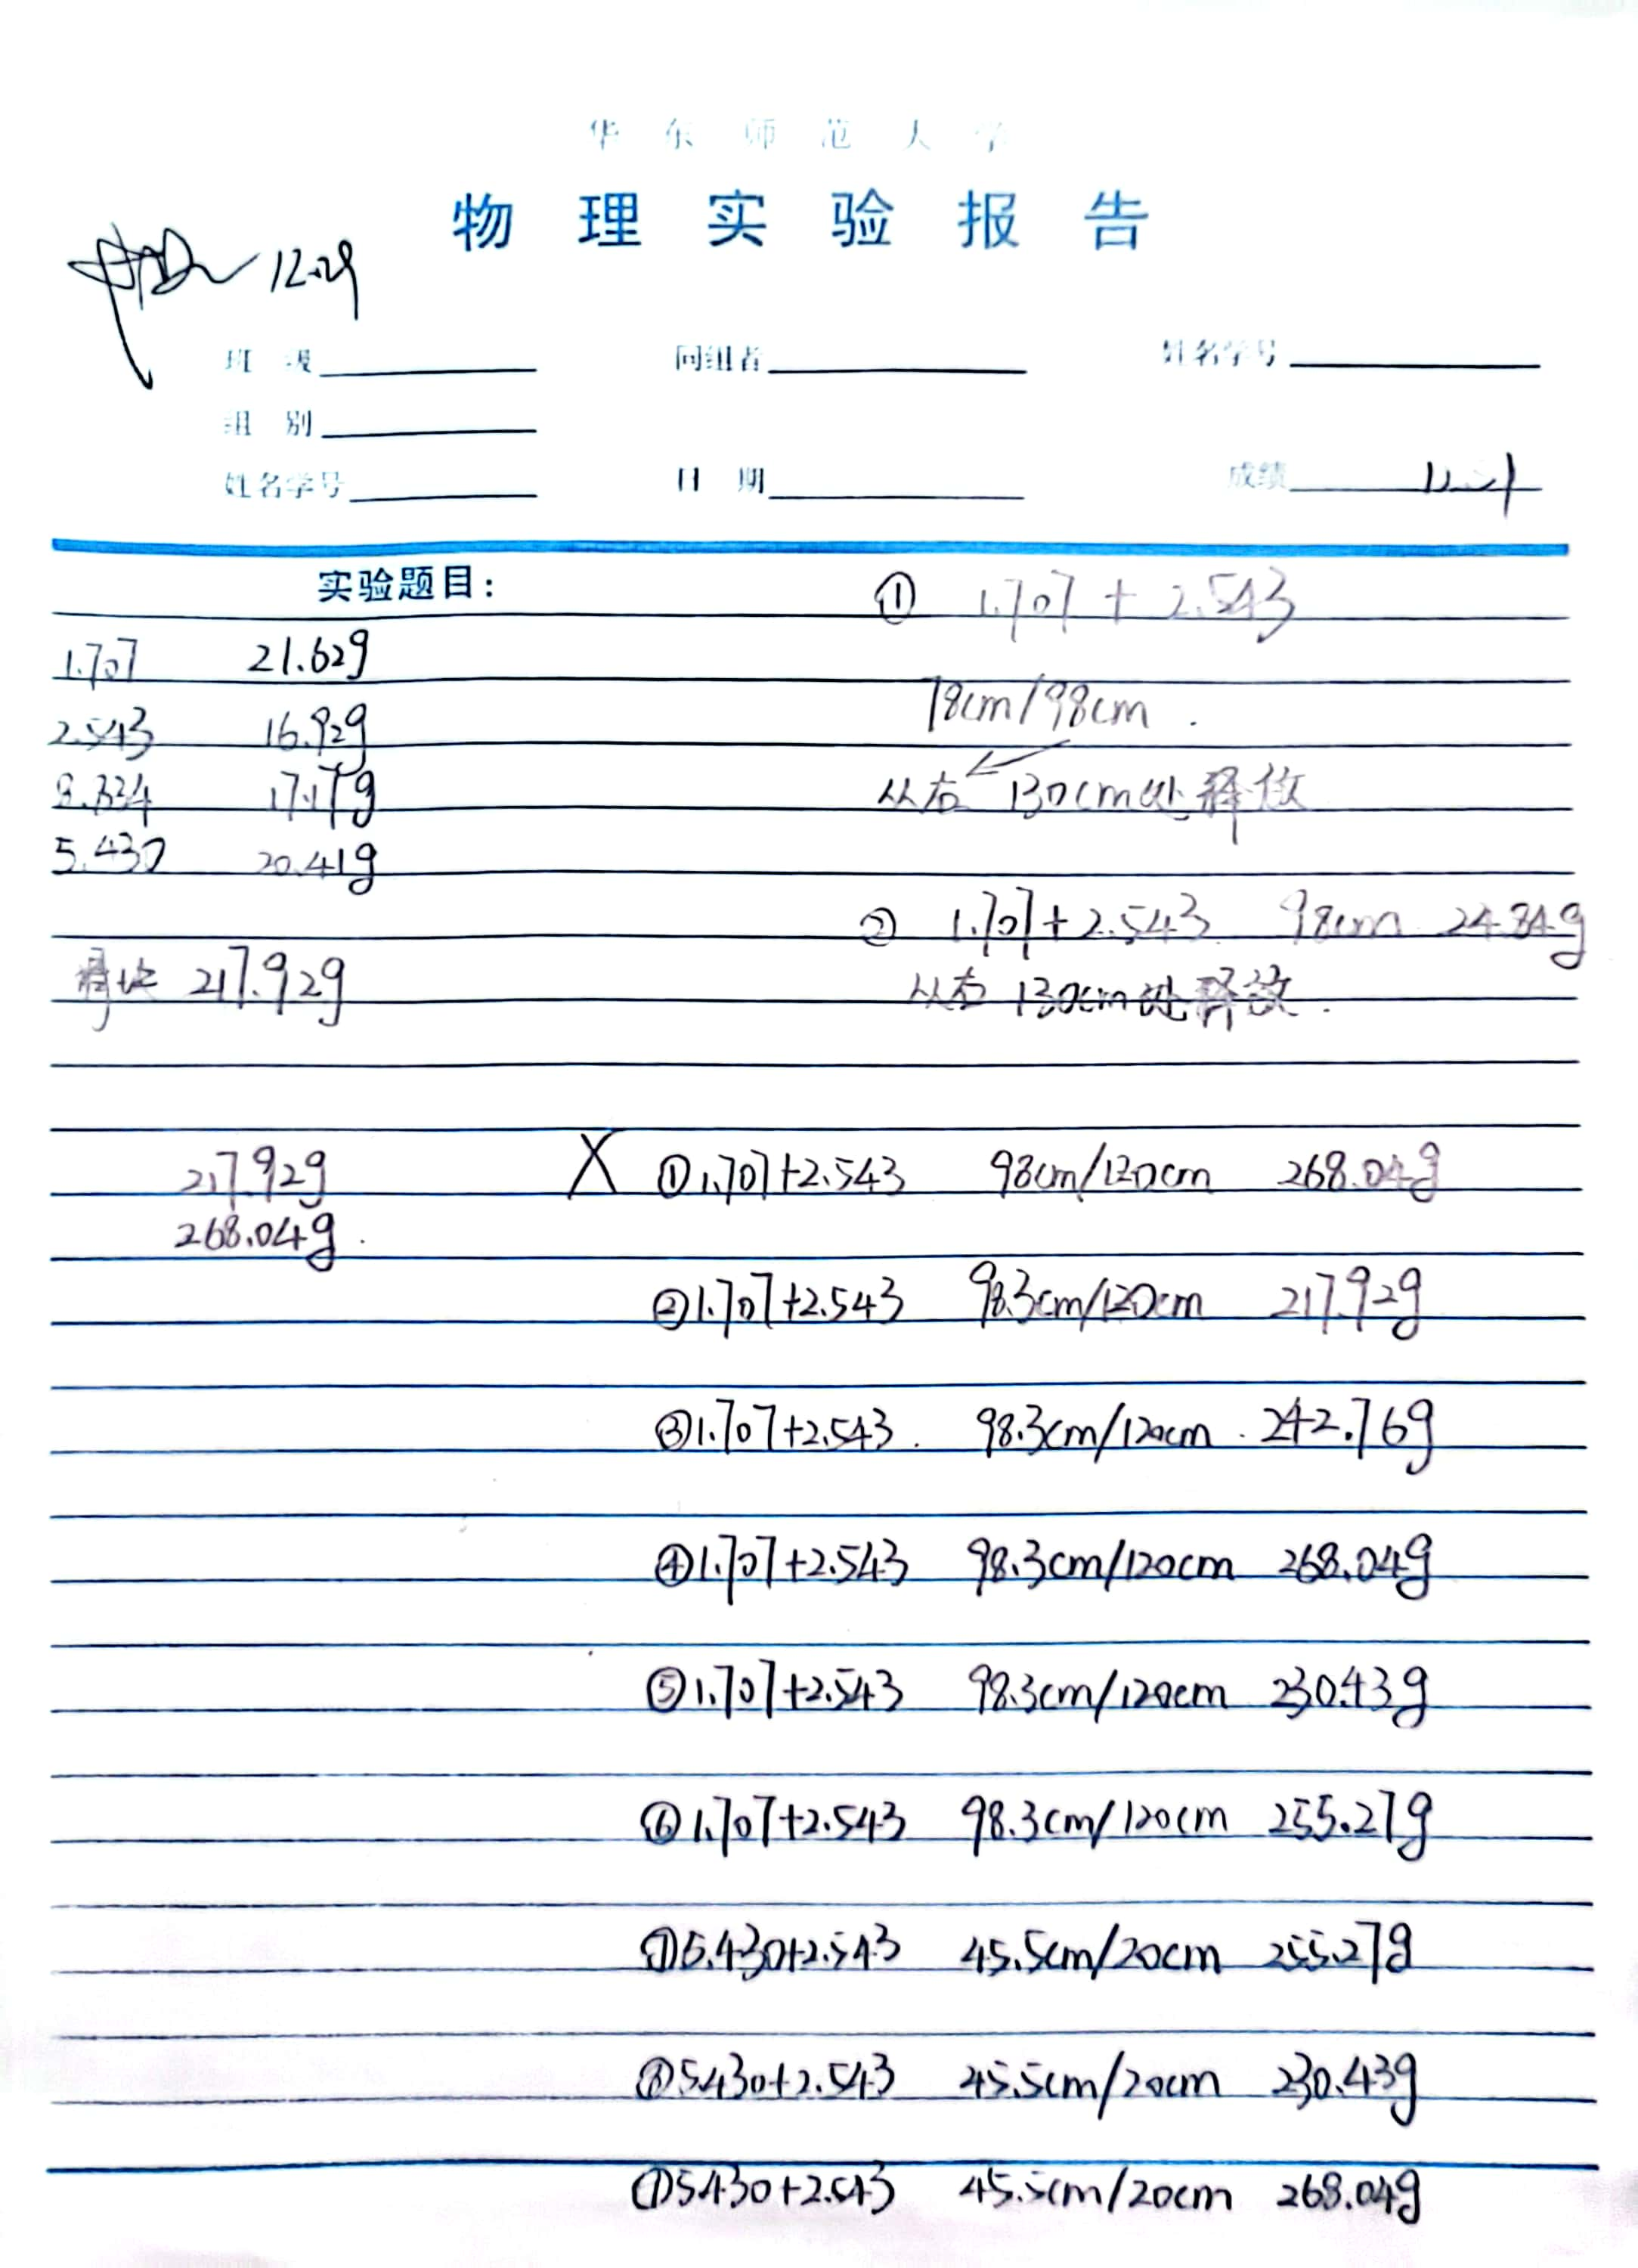
\includegraphics[width=0.9\textwidth,height=0.85\textheight]{shujvchuli0.jpg}
  \caption{原始数据0}
\end{figure}


\begin{figure}[H]
  \centering
  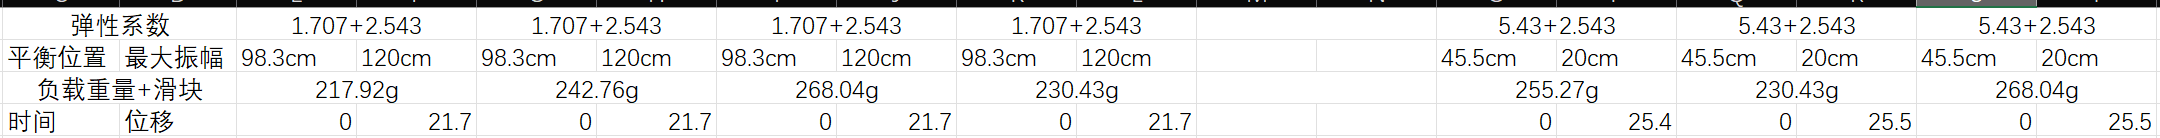
\includegraphics[width=0.95\textwidth,height=0.05\textheight]{shujvchuli1.png}
  \caption{原始数据1}
\end{figure}

\begin{figure}[H]
  \centering
  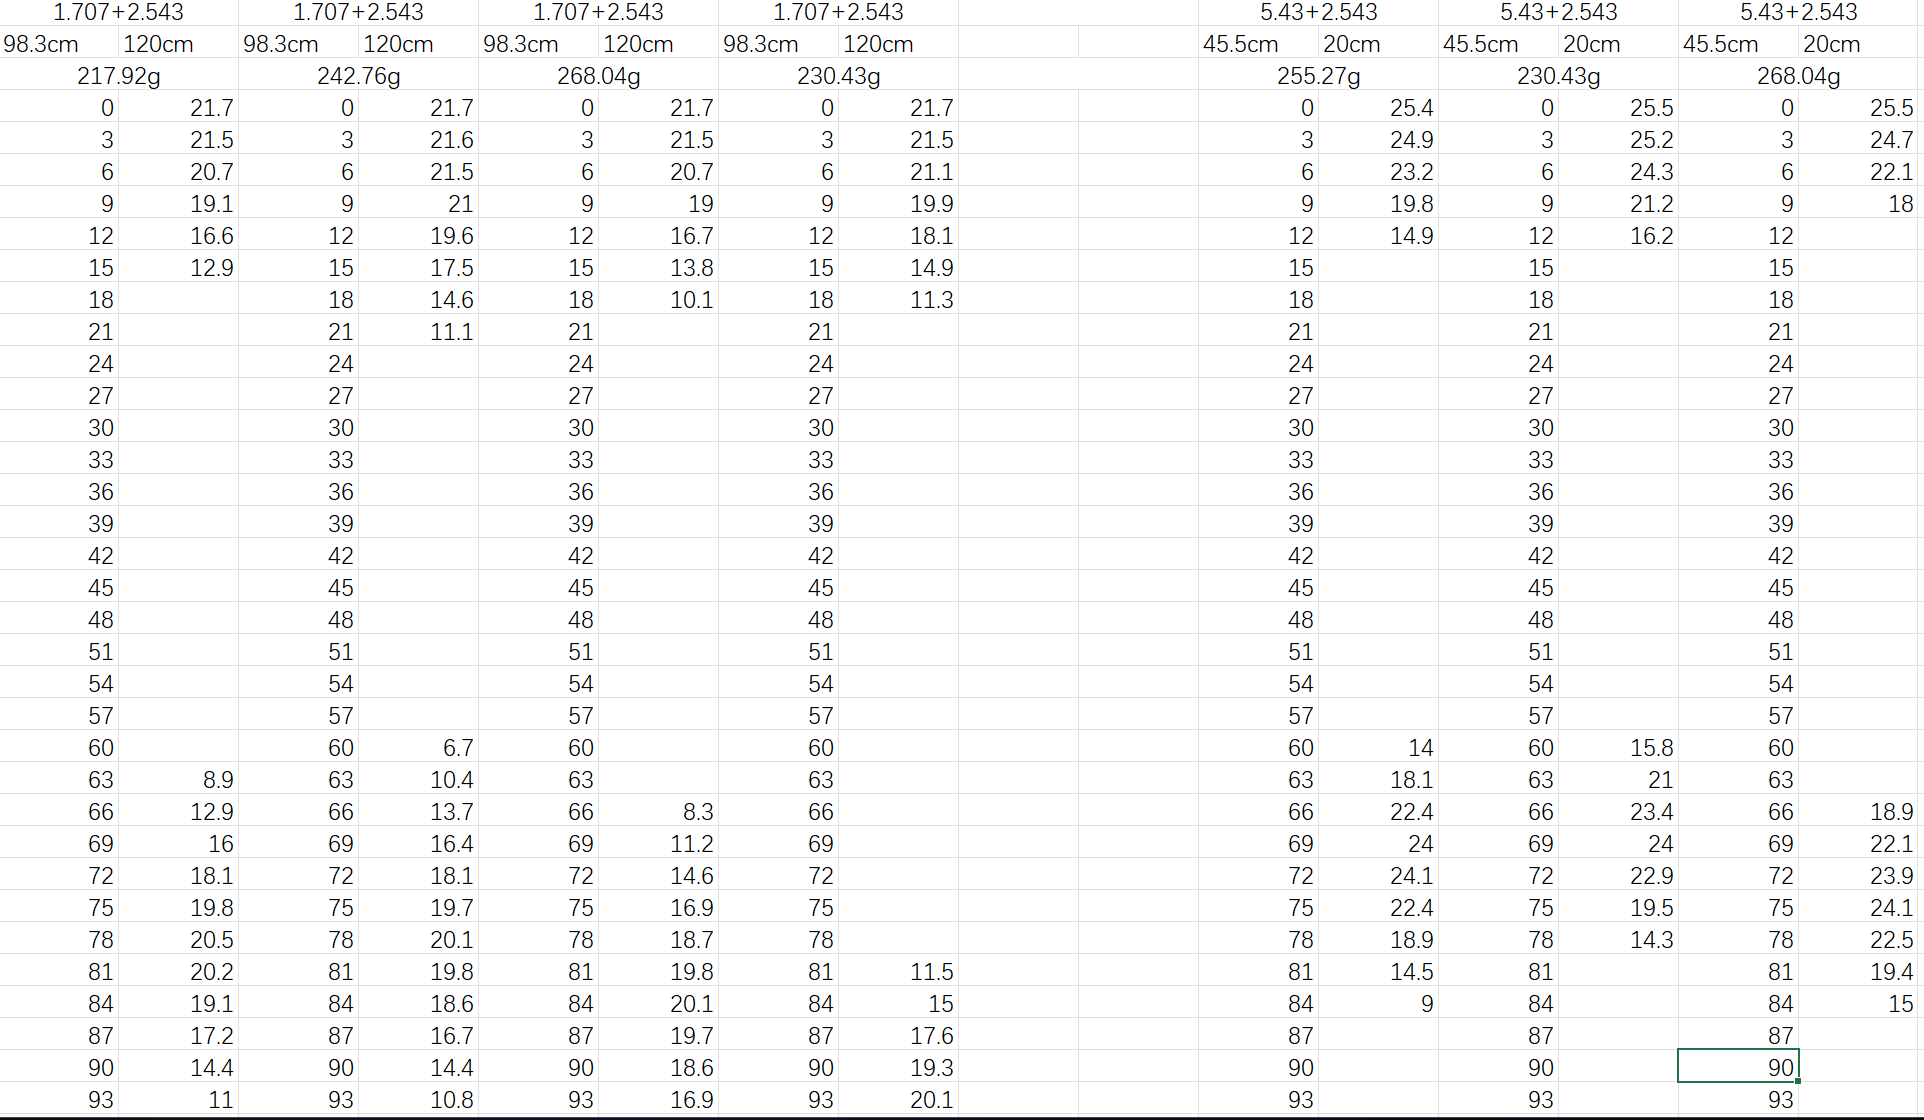
\includegraphics[width=0.85\textwidth,height=0.6\textheight]{shujvchuli2.png}
  \caption{原始数据2}
\end{figure}
\newpage
%----------------------------------------------------------------------------------------
\begin{figure}[H]
  \centering
  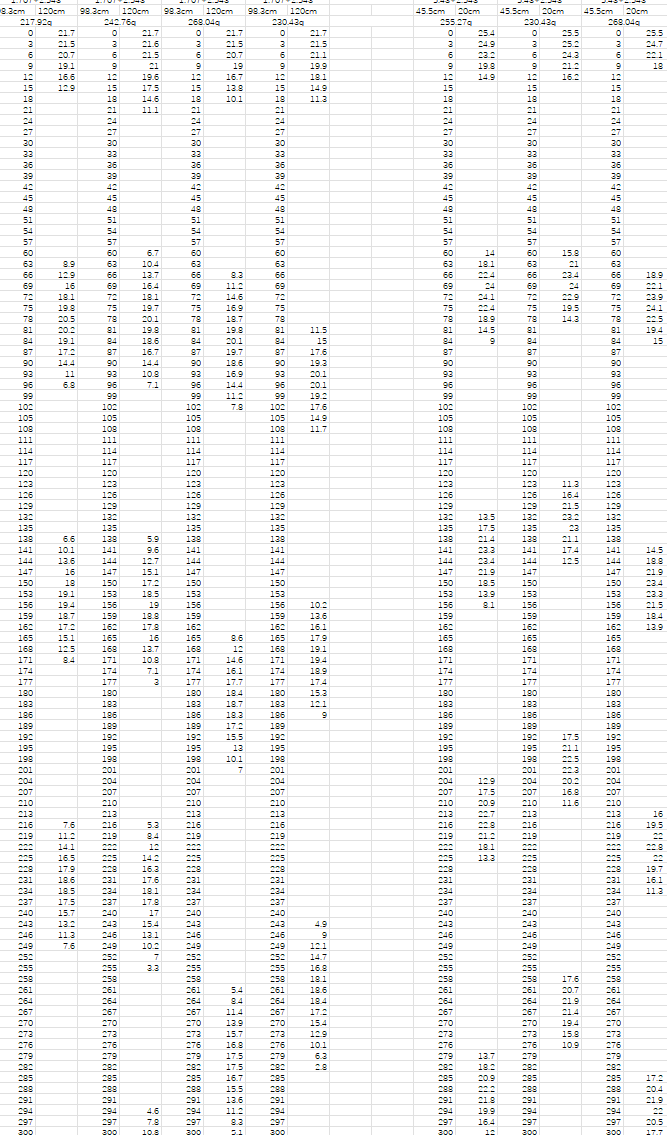
\includegraphics[width=0.8\textwidth,height=0.9\textheight]{shujvchuli3.png}
  \caption{原始数据3}
\end{figure}

由于数据过长,所以只截取了部分数据进行展示。
\newpage
%----------------------------------------------------------------------------------------

\section{数据处理}

  \subsection{数据对应关系}
  实验中使用的弹簧及其质量如表\ref{tanhuang}所示。
  \begin{table}[H]
    \centering   
    \caption{弹簧弹性系数及该系数弹簧的质量对应关系示意图}\label{tanhuang}
    \begin{tabular}{| l || l |}
        \hline
        弹簧的弹性系数 & 弹簧质量(克)\\
        \hline
        1.707 & 21.62 \\
        \hline
        2.543 & 16.92 \\
        \hline
        8.834 & 17.17 \\
        \hline
        5.430 & 20.41 \\
        \hline                       
    \end{tabular}
  \end{table}

  实验得到的数据可视化处理后得到的图像和对应关系如表\ref{guanxi}所示。
  \begin{table}[H]
    \centering   
    \caption{系列序号以及实验条件}\label{guanxi}
    \begin{tabular}{| c || c || c |}
        \hline
        系列序号 & 所使用弹簧 & 质量(克)\\
        \hline
        1 & 1.707+2.543 & 217.92\\
        \hline
        2 & 1.707+2.543 & 242.76\\
        \hline
        3 & 1.707+2.543 & 268.04\\
        \hline
        4 & 1.707+2.543 & 230.43\\
        \hline
        5 & 5.430+2.543 & 255.27\\
        \hline   
        6 & 5.430+2.543 & 230.43\\
        \hline
        7 & 5.430+2.543 & 268.04\\
        \hline                             
    \end{tabular}
  \end{table}

  \subsection{数据处理后图片展示}
  \begin{figure}[H]
    \centering
    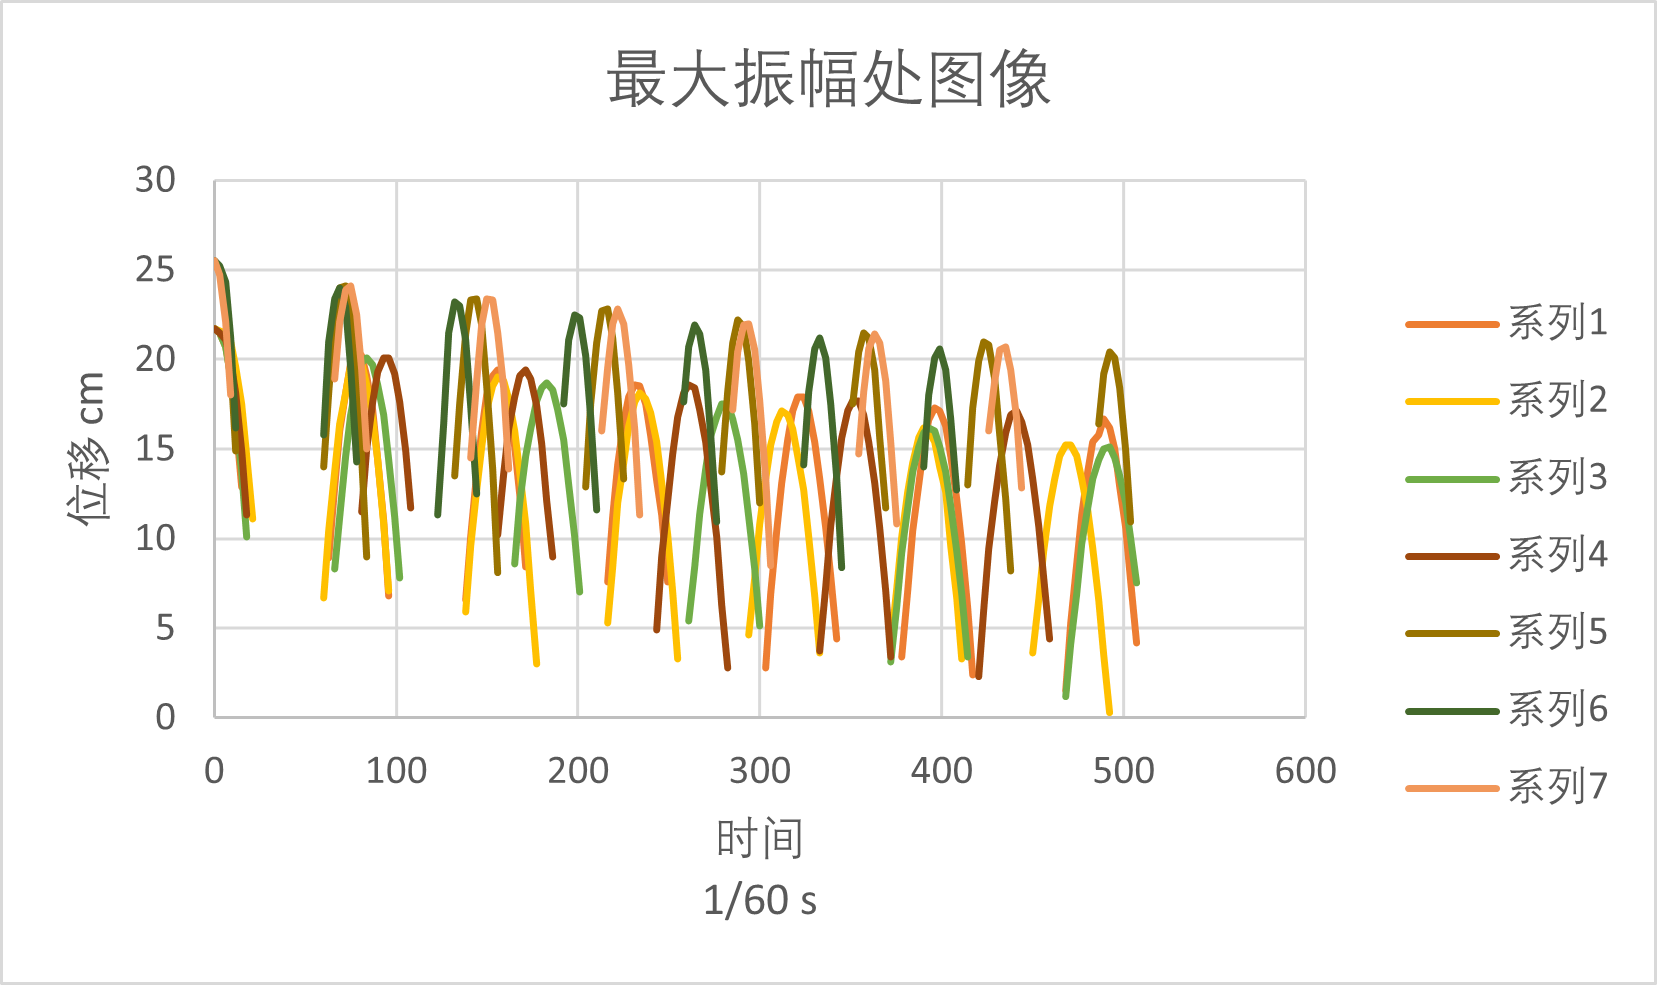
\includegraphics[width=0.85\textwidth,height=0.6\textheight]{tuxiangquan.png}
    \caption{处理后图像(全)}
  \end{figure}
  \newpage
  %----------------------------------------------------------------------------------------
  以下图片展示的是相同振幅释放后,相同弹簧弹性系数的条件下不同滑块质量的结果:

  \begin{figure}[H]
    \centering
    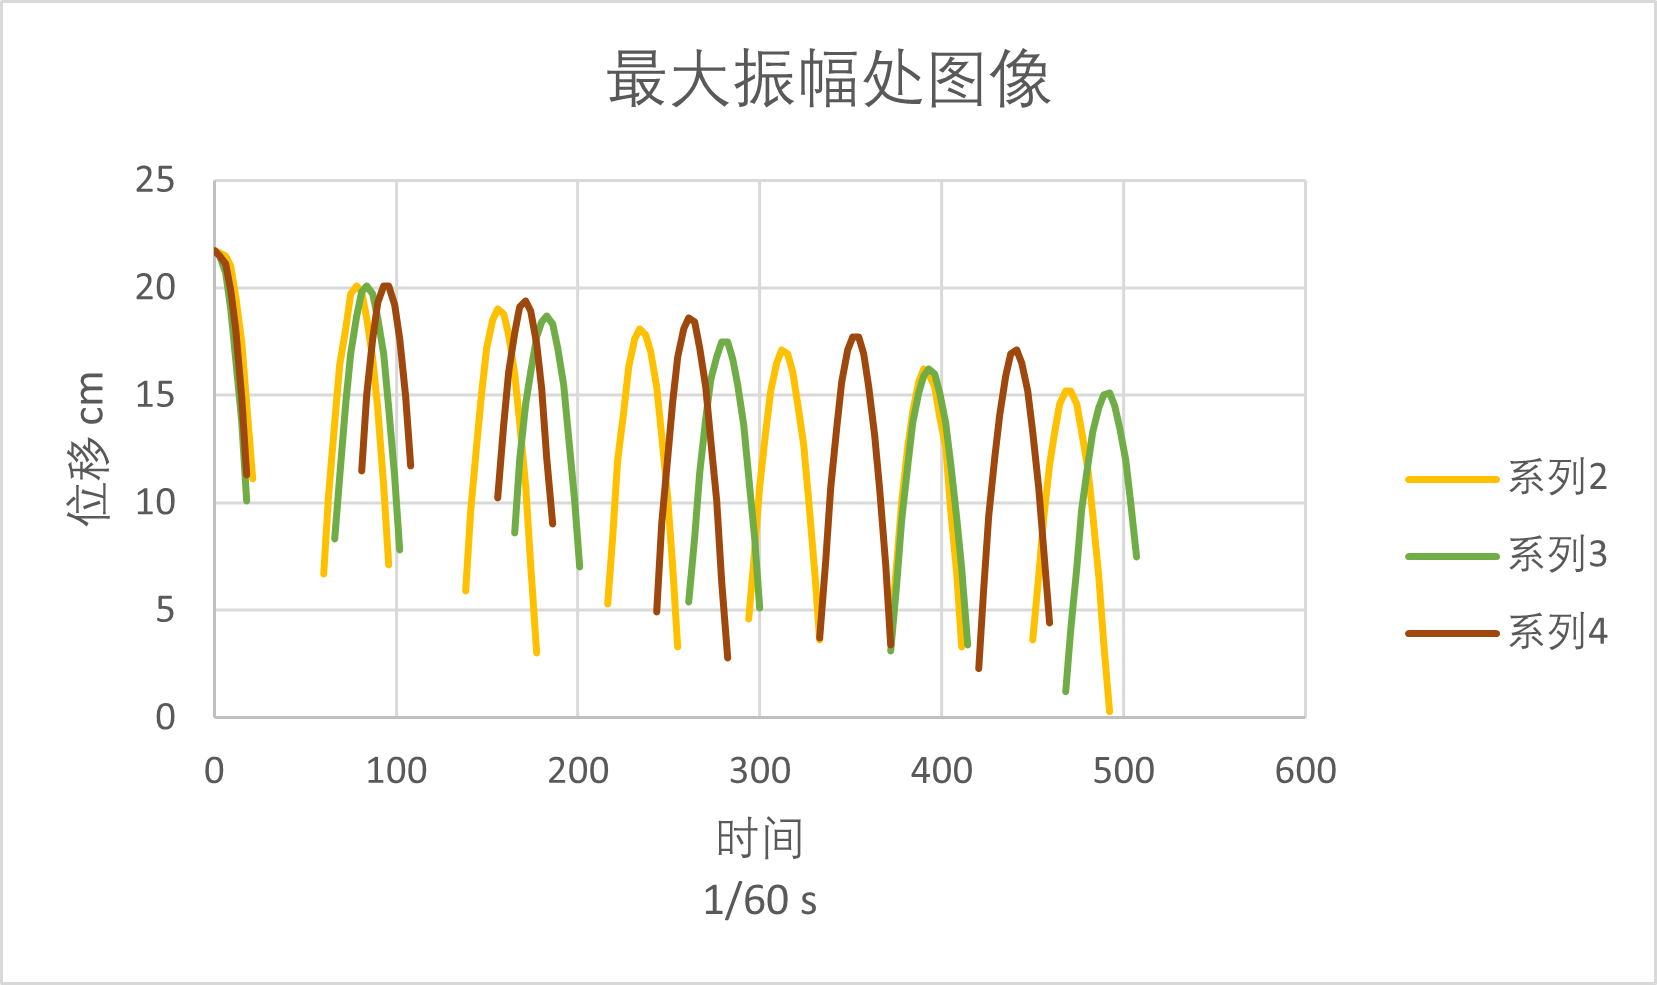
\includegraphics[width=0.65\textwidth,height=0.35\textheight]{zhiliang1.png}
    \caption{数据图像1}
  \end{figure}

  \begin{figure}[H]
    \centering
    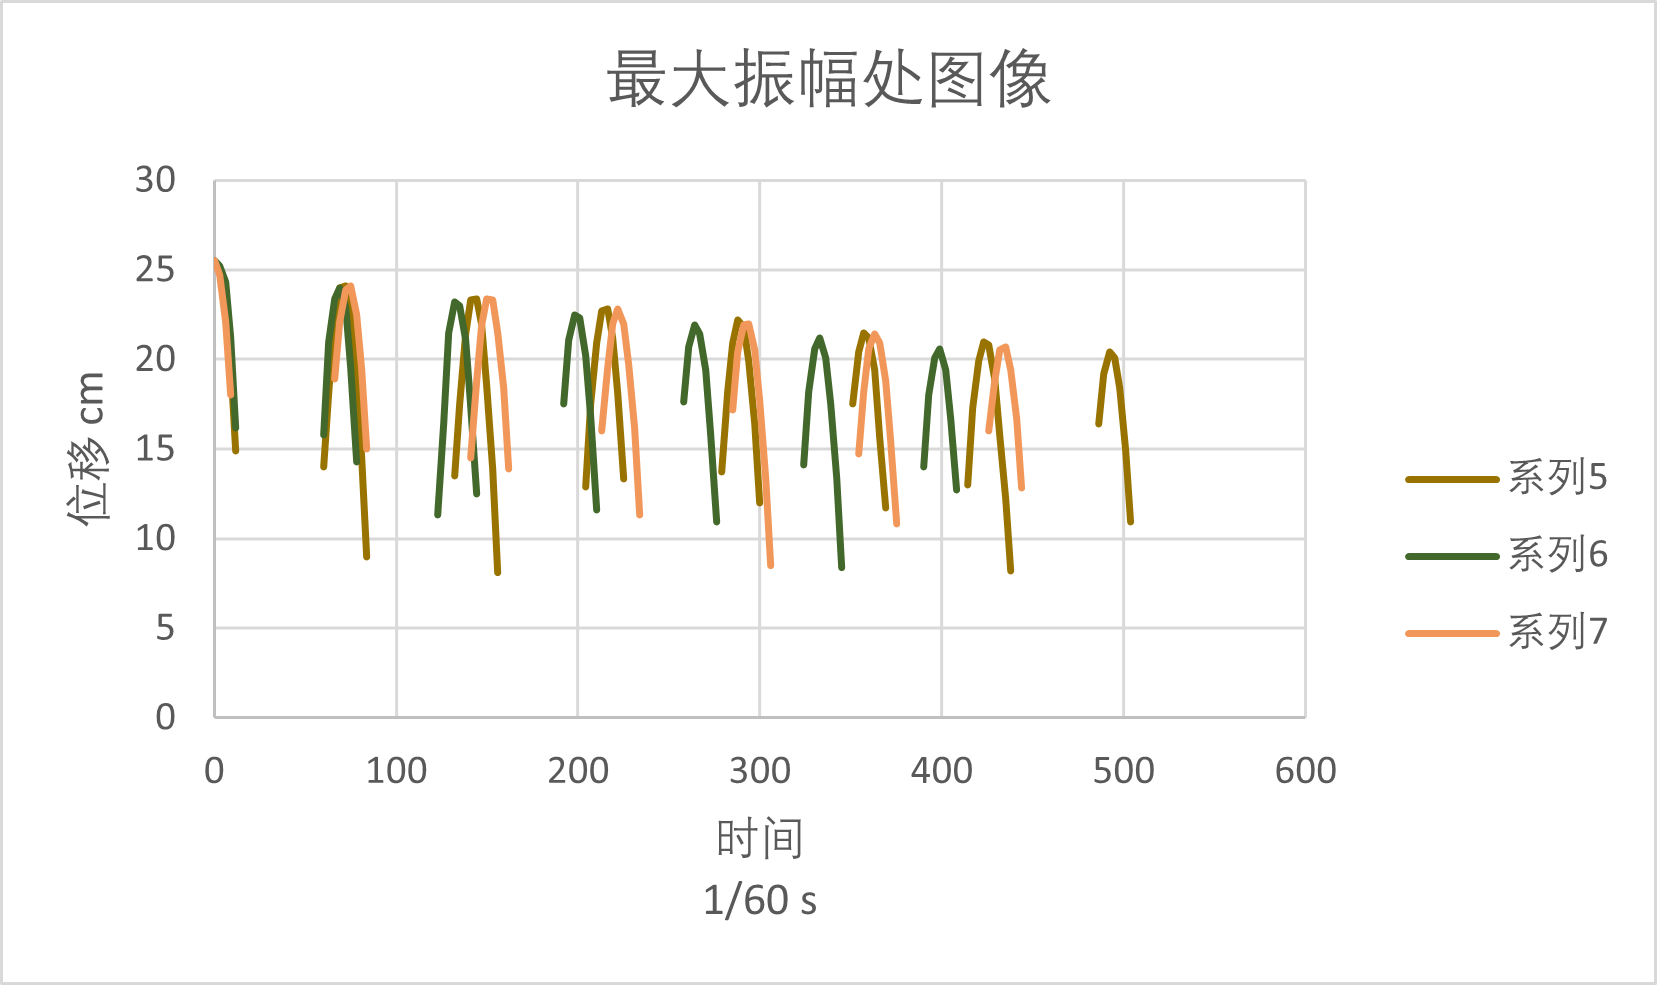
\includegraphics[width=0.65\textwidth,height=0.35\textheight]{zhiliang2.png}
    \caption{数据图像2}
  \end{figure}
  \newpage
  %----------------------------------------------------------------------------------------
  以下图片展示的是不同弹簧弹性系数的条件下相同滑块质量的结果:
  \begin{figure}[H]
    \centering
    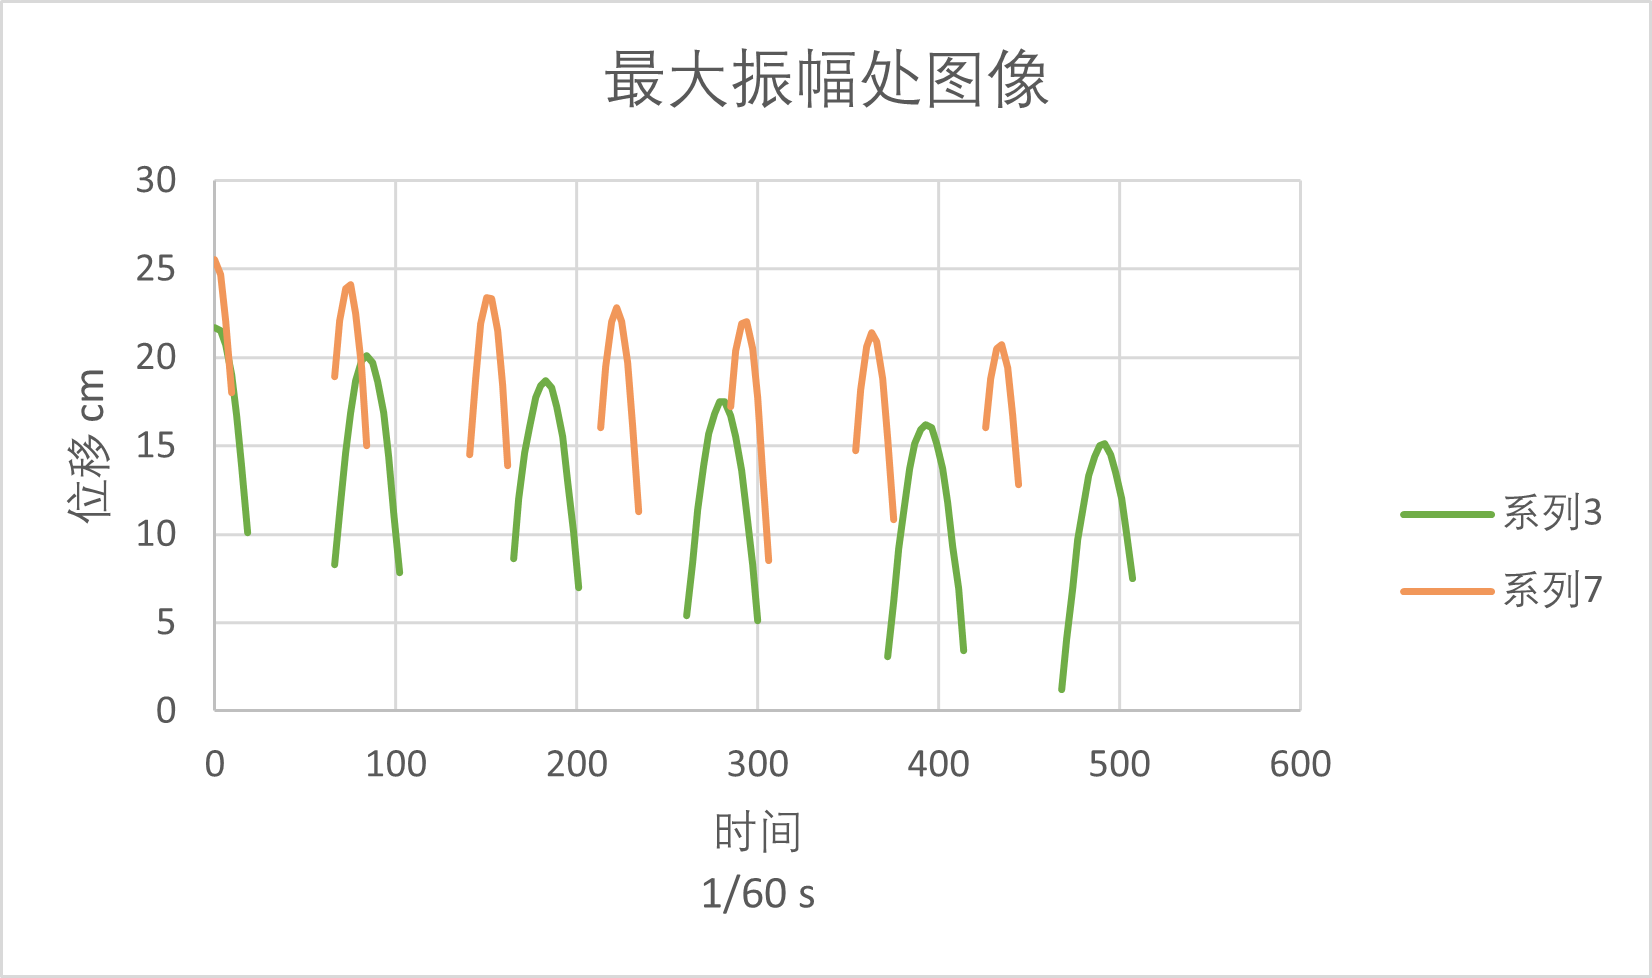
\includegraphics[width=0.65\textwidth,height=0.4\textheight]{tanhuang1.png}
    \caption{数据图像3}
  \end{figure}

  \begin{figure}[H]
    \centering
    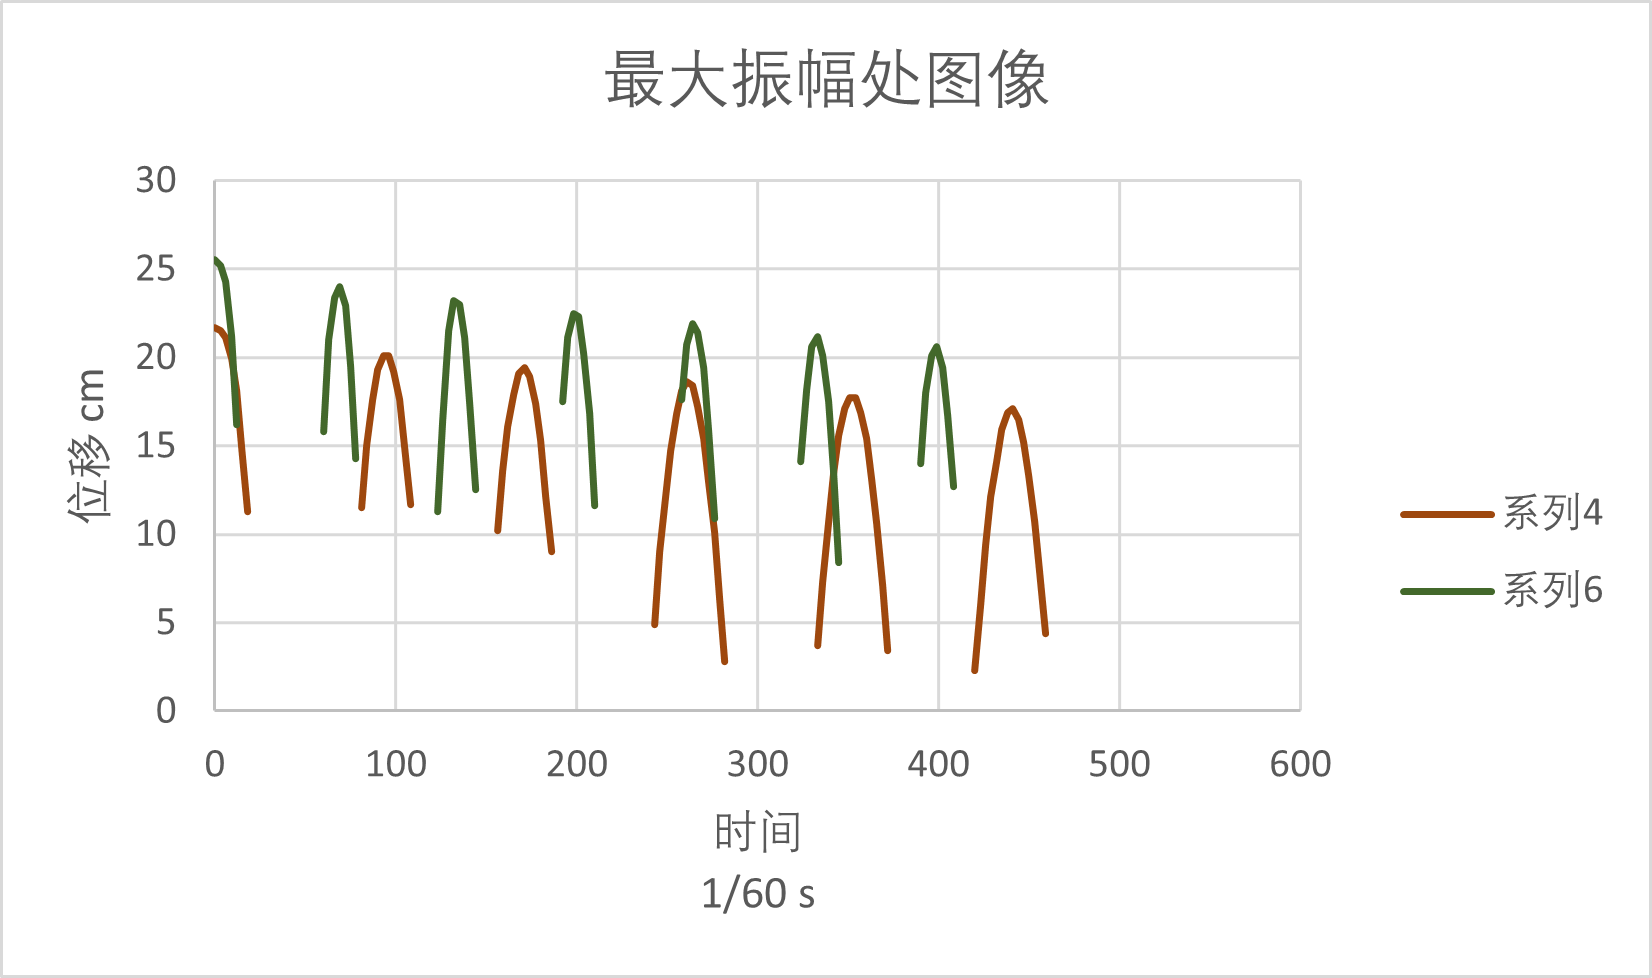
\includegraphics[width=0.65\textwidth,height=0.4\textheight]{tanhuang2.png}
    \caption{数据图像4}
  \end{figure}
  \newpage
  %----------------------------------------------------------------------------------------

  \subsection{相关数据计算}
  进行计算后可以得到实验所需要的相关值的大小,如表\ref{jisuan}所示。

  \begin{table}[H]
    \centering   
    \caption{系列以及相关实验值计算}\label{jisuan}
    \begin{tabular}{| c || c || c || c |}
        \hline
        系列序号 & b & $\Delta$ & Q\\
        \hline
        1 & 17.22 & 0.0395 & 60.39\\
        \hline
        2 & 26.75 & 0.0551 & 43.86\\
        \hline
        3 & 29.33 & 0.0547 & 41.02\\
        \hline
        4 & 21.07 & 0.0457 & 43.86\\
        \hline
        5 & 22.90 & 0.0449 & 60.04\\
        \hline   
        6 & 24.29 & 0.0527 & 51.82\\
        \hline
        7 & 21.86 & 0.0408 & 60.04\\
        \hline                             
    \end{tabular}
  \end{table}

  \subsection{误差分析}
  \begin{table}[H]
    \centering   
    \caption{误差分析}
    \begin{tabular}{| c || c || c |}
        \hline
        系列序号 & 振幅(米) & 质量(千克)\\
        \hline
        1 & 0.00067 & 0.00582\\
        \hline
        2 & 0.00067 & 0.00582\\
        \hline
        3 & 0.00067 & 0.00582\\
        \hline
        4 & 0.00067 & 0.00582\\
        \hline
        5 & 0.00067 & 0.00582\\
        \hline   
        6 & 0.00067 & 0.00582\\
        \hline
        7 & 0.00067 & 0.00582\\
        \hline                             
    \end{tabular}
  \end{table}
\newpage


\section{实验结论}
  最终实验可以得出阻尼振动中周期随着质量增加而增加,振幅随着时间增加而减小。如图\ref{tuxiang1}和图\ref{tuxiang2}所示。
  \begin{figure}[H]
    \centering 
    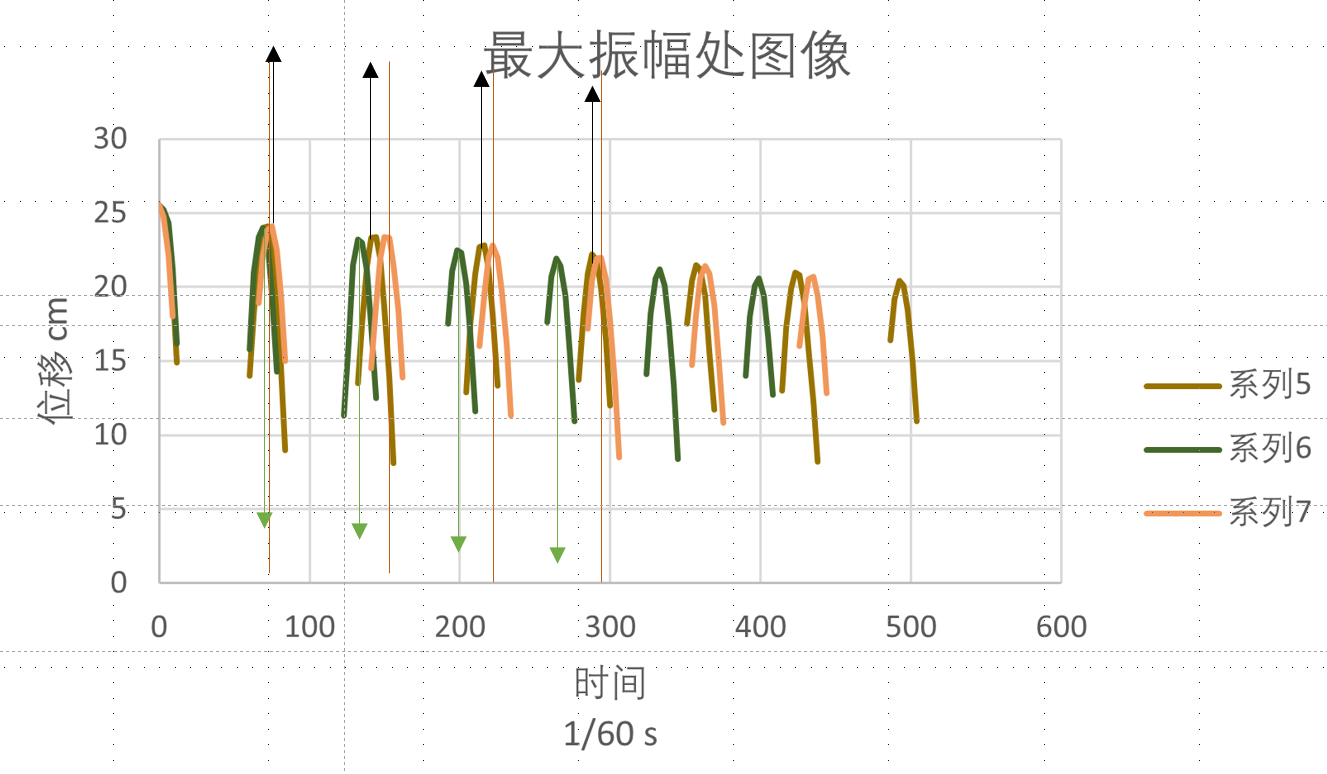
\includegraphics[width=0.65\textwidth,height=0.35\textheight]{tuxaing1.png}
    \caption{图像1}
    \label{tuxiang1}
  \end{figure}

  \begin{figure}[H]
    \centering 
    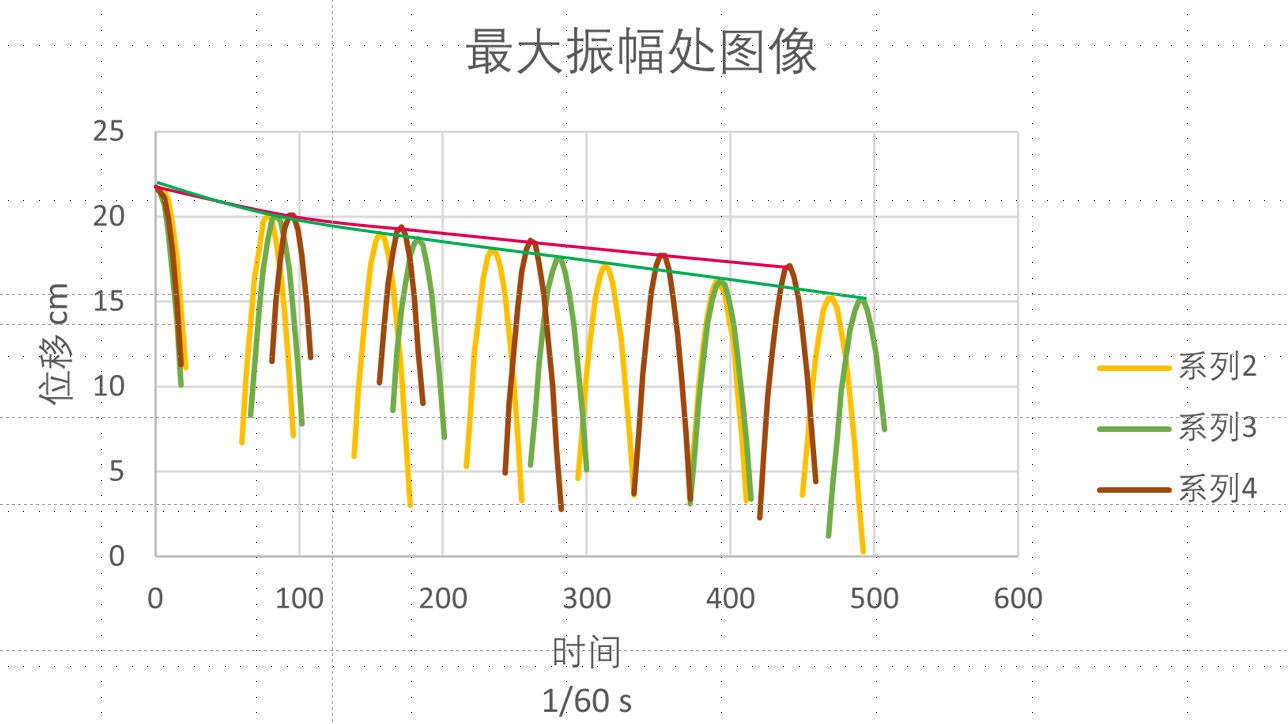
\includegraphics[width=0.65\textwidth,height=0.35\textheight]{tuxiang2.png}
    \caption{图像2}
    \label{tuxiang2}
  \end{figure}

  同时计算得到了实验中所使用设备条件下的品质因数与阻尼系数。

  实验能够定性表现出阻尼振动和滑块质量与弹簧弹性系数的关系。

\section{实验讨论}
  实验中有很多容易导致误差的地方。比如弹簧在振动的时候可能会左右晃动导致即便没有阻尼也不是简谐振动。而且气垫导轨不同位置的喷气力度不同也导致饰演的误差。

  之前拿这套相同的设备进行过简谐振动的实验,通过这次实验会感觉上一次实验的误差非常大,而事实上是之前实验中的确也遇到了误差过大的问题。
  所以这次实验或许也算是解释之前实验中误差分析中解释的“可能由于不是理想的简谐振动”的补充。
  
\end{document}